%%
%% Automatically generated file from DocOnce source
%% (https://github.com/doconce/doconce/)
%% doconce format latex week3.do.txt --latex_title_layout=beamer --latex_table_format=footnotesize --no_mako
%%
% #ifdef PTEX2TEX_EXPLANATION
%%
%% The file follows the ptex2tex extended LaTeX format, see
%% ptex2tex: https://code.google.com/p/ptex2tex/
%%
%% Run
%%      ptex2tex myfile
%% or
%%      doconce ptex2tex myfile
%%
%% to turn myfile.p.tex into an ordinary LaTeX file myfile.tex.
%% (The ptex2tex program: https://code.google.com/p/ptex2tex)
%% Many preprocess options can be added to ptex2tex or doconce ptex2tex
%%
%%      ptex2tex -DMINTED myfile
%%      doconce ptex2tex myfile envir=minted
%%
%% ptex2tex will typeset code environments according to a global or local
%% .ptex2tex.cfg configure file. doconce ptex2tex will typeset code
%% according to options on the command line (just type doconce ptex2tex to
%% see examples). If doconce ptex2tex has envir=minted, it enables the
%% minted style without needing -DMINTED.
% #endif

% #define PREAMBLE

% #ifdef PREAMBLE
%-------------------- begin preamble ----------------------

\documentclass[%
oneside,                 % oneside: electronic viewing, twoside: printing
final,                   % draft: marks overfull hboxes, figures with paths
10pt]{article}

\listfiles               %  print all files needed to compile this document

\usepackage{relsize,makeidx,color,setspace,amsmath,amsfonts,amssymb}
\usepackage[table]{xcolor}
\usepackage{bm,ltablex,microtype}

\usepackage[pdftex]{graphicx}

\usepackage{ptex2tex}
% #ifdef MINTED
\usepackage{minted}
\usemintedstyle{default}
% #endif

\usepackage[T1]{fontenc}
%\usepackage[latin1]{inputenc}
\usepackage{ucs}
\usepackage[utf8x]{inputenc}

\usepackage{lmodern}         % Latin Modern fonts derived from Computer Modern

% Hyperlinks in PDF:
\definecolor{linkcolor}{rgb}{0,0,0.4}
\usepackage{hyperref}
\hypersetup{
    breaklinks=true,
    colorlinks=true,
    linkcolor=linkcolor,
    urlcolor=linkcolor,
    citecolor=black,
    filecolor=black,
    %filecolor=blue,
    pdfmenubar=true,
    pdftoolbar=true,
    bookmarksdepth=3   % Uncomment (and tweak) for PDF bookmarks with more levels than the TOC
    }
%\hyperbaseurl{}   % hyperlinks are relative to this root

\setcounter{tocdepth}{2}  % levels in table of contents

% Tricks for having figures close to where they are defined:
% 1. define less restrictive rules for where to put figures
\setcounter{topnumber}{2}
\setcounter{bottomnumber}{2}
\setcounter{totalnumber}{4}
\renewcommand{\topfraction}{0.95}
\renewcommand{\bottomfraction}{0.95}
\renewcommand{\textfraction}{0}
\renewcommand{\floatpagefraction}{0.75}
% floatpagefraction must always be less than topfraction!
% 2. ensure all figures are flushed before next section
\usepackage[section]{placeins}
% 3. enable begin{figure}[H] (often leads to ugly pagebreaks)
%\usepackage{float}\restylefloat{figure}

% --- fancyhdr package for fancy headers ---
\usepackage{fancyhdr}
\fancyhf{} % sets both header and footer to nothing
\renewcommand{\headrulewidth}{0pt}
\fancyfoot[LE,RO]{\thepage}
% Ensure copyright on titlepage (article style) and chapter pages (book style)
\fancypagestyle{plain}{
  \fancyhf{}
  \fancyfoot[C]{{\footnotesize \copyright\ 1999-2024, Morten Hjorth-Jensen. Released under CC Attribution-NonCommercial 4.0 license}}
%  \renewcommand{\footrulewidth}{0mm}
  \renewcommand{\headrulewidth}{0mm}
}
% Ensure copyright on titlepages with \thispagestyle{empty}
\fancypagestyle{empty}{
  \fancyhf{}
  \fancyfoot[C]{{\footnotesize \copyright\ 1999-2024, Morten Hjorth-Jensen. Released under CC Attribution-NonCommercial 4.0 license}}
  \renewcommand{\footrulewidth}{0mm}
  \renewcommand{\headrulewidth}{0mm}
}

\pagestyle{fancy}


\usepackage[framemethod=TikZ]{mdframed}

% --- begin definitions of admonition environments ---

% Admonition style "mdfbox" is an oval colored box based on mdframed
% "notice" admon
\colorlet{mdfbox_notice_background}{gray!5}
\newmdenv[
  skipabove=15pt,
  skipbelow=15pt,
  outerlinewidth=0,
  backgroundcolor=mdfbox_notice_background,
  linecolor=black,
  linewidth=2pt,       % frame thickness
  frametitlebackgroundcolor=mdfbox_notice_background,
  frametitlerule=true,
  frametitlefont=\normalfont\bfseries,
  shadow=false,        % frame shadow?
  shadowsize=11pt,
  leftmargin=0,
  rightmargin=0,
  roundcorner=5,
  needspace=0pt,
]{notice_mdfboxmdframed}

\newenvironment{notice_mdfboxadmon}[1][]{
\begin{notice_mdfboxmdframed}[frametitle=#1]
}
{
\end{notice_mdfboxmdframed}
}

% Admonition style "mdfbox" is an oval colored box based on mdframed
% "summary" admon
\colorlet{mdfbox_summary_background}{gray!5}
\newmdenv[
  skipabove=15pt,
  skipbelow=15pt,
  outerlinewidth=0,
  backgroundcolor=mdfbox_summary_background,
  linecolor=black,
  linewidth=2pt,       % frame thickness
  frametitlebackgroundcolor=mdfbox_summary_background,
  frametitlerule=true,
  frametitlefont=\normalfont\bfseries,
  shadow=false,        % frame shadow?
  shadowsize=11pt,
  leftmargin=0,
  rightmargin=0,
  roundcorner=5,
  needspace=0pt,
]{summary_mdfboxmdframed}

\newenvironment{summary_mdfboxadmon}[1][]{
\begin{summary_mdfboxmdframed}[frametitle=#1]
}
{
\end{summary_mdfboxmdframed}
}

% Admonition style "mdfbox" is an oval colored box based on mdframed
% "warning" admon
\colorlet{mdfbox_warning_background}{gray!5}
\newmdenv[
  skipabove=15pt,
  skipbelow=15pt,
  outerlinewidth=0,
  backgroundcolor=mdfbox_warning_background,
  linecolor=black,
  linewidth=2pt,       % frame thickness
  frametitlebackgroundcolor=mdfbox_warning_background,
  frametitlerule=true,
  frametitlefont=\normalfont\bfseries,
  shadow=false,        % frame shadow?
  shadowsize=11pt,
  leftmargin=0,
  rightmargin=0,
  roundcorner=5,
  needspace=0pt,
]{warning_mdfboxmdframed}

\newenvironment{warning_mdfboxadmon}[1][]{
\begin{warning_mdfboxmdframed}[frametitle=#1]
}
{
\end{warning_mdfboxmdframed}
}

% Admonition style "mdfbox" is an oval colored box based on mdframed
% "question" admon
\colorlet{mdfbox_question_background}{gray!5}
\newmdenv[
  skipabove=15pt,
  skipbelow=15pt,
  outerlinewidth=0,
  backgroundcolor=mdfbox_question_background,
  linecolor=black,
  linewidth=2pt,       % frame thickness
  frametitlebackgroundcolor=mdfbox_question_background,
  frametitlerule=true,
  frametitlefont=\normalfont\bfseries,
  shadow=false,        % frame shadow?
  shadowsize=11pt,
  leftmargin=0,
  rightmargin=0,
  roundcorner=5,
  needspace=0pt,
]{question_mdfboxmdframed}

\newenvironment{question_mdfboxadmon}[1][]{
\begin{question_mdfboxmdframed}[frametitle=#1]
}
{
\end{question_mdfboxmdframed}
}

% Admonition style "mdfbox" is an oval colored box based on mdframed
% "block" admon
\colorlet{mdfbox_block_background}{gray!5}
\newmdenv[
  skipabove=15pt,
  skipbelow=15pt,
  outerlinewidth=0,
  backgroundcolor=mdfbox_block_background,
  linecolor=black,
  linewidth=2pt,       % frame thickness
  frametitlebackgroundcolor=mdfbox_block_background,
  frametitlerule=true,
  frametitlefont=\normalfont\bfseries,
  shadow=false,        % frame shadow?
  shadowsize=11pt,
  leftmargin=0,
  rightmargin=0,
  roundcorner=5,
  needspace=0pt,
]{block_mdfboxmdframed}

\newenvironment{block_mdfboxadmon}[1][]{
\begin{block_mdfboxmdframed}[frametitle=#1]
}
{
\end{block_mdfboxmdframed}
}

% --- end of definitions of admonition environments ---

% prevent orhpans and widows
\clubpenalty = 10000
\widowpenalty = 10000

% --- end of standard preamble for documents ---


% insert custom LaTeX commands...

\raggedbottom
\makeindex

%-------------------- end preamble ----------------------

\begin{document}

% matching end for #ifdef PREAMBLE
% #endif

\newcommand{\exercisesection}[1]{\subsection*{#1}}


% ------------------- main content ----------------------



% ----------------- title -------------------------

\title{January 29-February 2 : Advanced machine learning and data analysis for the physical sciences}

% ----------------- author(s) -------------------------

\author{Morten Hjorth-Jensen\inst{1,2}}
\institute{Department of Physics and Center for Computing in Science Education, University of Oslo, Norway\inst{1}
\and
Department of Physics and Astronomy and Facility for Rare Isotope Beams, Michigan State University, East Lansing, Michigan, USA\inst{2}}
% ----------------- end author(s) -------------------------

\date{January 30
% <optional titlepage figure>
% <optional copyright>
}

% !split
\subsection{Overview of third  week}

\begin{block}{}
\begin{enumerate}
 \item Discussion of possible projects

 \item Review of neural networks and automatic differentiation

 \item Discussion of codes
\end{enumerate}

\noindent
\end{block}

% !split
\subsection{Mathematics of deep learning}

\begin{block}{Two recent books online }
\begin{enumerate}
\item \href{{https://arxiv.org/abs/2105.04026}}{The Modern Mathematics of Deep Learning, by Julius Berner, Philipp Grohs, Gitta Kutyniok, Philipp Petersen}, published as \href{{https://doi.org/10.1017/9781009025096.002}}{Mathematical Aspects of Deep Learning, pp. 1-111. Cambridge University Press, 2022}

\item \href{{https://doi.org/10.48550/arXiv.2310.20360}}{Mathematical Introduction to Deep Learning: Methods, Implementations, and Theory, Arnulf Jentzen, Benno Kuckuck, Philippe von Wurstemberger}
\end{enumerate}

\noindent
\end{block}

% !split
\subsection{Reminder on books with hands-on material and codes}
\begin{block}{}
\begin{itemize}
\item \href{{https://sebastianraschka.com/blog/2022/ml-pytorch-book.html}}{Sebastian Rashcka et al, Machine learning with Sickit-Learn and PyTorch}

\item \href{{https://www.oreilly.com/library/view/generative-deep-learning/9781098134174/ch01.html}}{David Foster, Generative Deep Learning with TensorFlow}

\item \href{{https://github.com/PacktPublishing/Hands-On-Generative-AI-with-Python-and-TensorFlow-2}}{Bali and Gavras, Generative AI with Python and TensorFlow 2}
\end{itemize}

\noindent
\end{block}

All three books have GitHub addresses from where  one can download all codes. We will borrow most of the material from these three texts as well as 
from Goodfellow, Bengio and Courville's text \href{{https://www.deeplearningbook.org/}}{Deep Learning}

% !split
\subsection{Reading recommendations}

\begin{enumerate}
\item Rashkca et al., chapter 11, jupyter-notebook sent separately, from \href{{https://github.com/rasbt/machine-learning-book}}{GitHub}

\item Goodfellow et al, chapter 6 and 7 contain most of the neural network background.
\end{enumerate}

\noindent
% !split
\subsection{Mathematics of deep learning and neural networks}

Neural networks, in its so-called feed-forward form, where each
iterations contains a feed-forward stage and a back-propgagation
stage, consist of series of affine matrix-matrix and matrix-vector
multiplications. The unknown parameters (the so-called biases and
weights which deternine the architecture of a neural network), are
uptaded iteratively using the so-called back-propagation algorithm.
This algorithm corresponds to the so-called reverse mode of 
automatic differentation. 

% !split
\subsection{Basics of an NN}

A neural network consists of a series of hidden layers, in addition to
the input and output layers.  Each layer $l$ has a set of parameters
$\bm{\Theta}^{(l)}=(\bm{W}^{(l)},\bm{b}^{(l)})$ which are related to the
parameters in other layers through a series of affine transformations,
for a standard NN these are matrix-matrix and matrix-vector
multiplications.  For all layers we will simply use a collective variable $\bm{\Theta}$.

It consist of two basic steps:
\begin{enumerate}
\item a feed forward stage which takes a given input and produces a final output which is compared with the target values through our cost/loss function.

\item a back-propagation state where the unknown parameters $\bm{\Theta}$ are updated through the optimization of the their gradients. The expressions for the gradients are obtained via the chain rule, starting from the derivative of the cost/function.
\end{enumerate}

\noindent
These two steps make up one iteration. This iterative process is continued till we reach an eventual stopping criterion.

% !split
\subsection{Overarching view of a neural network}

The architecture of a neural network defines our model. This model
aims at describing some function $f(\bm{x}$ which represents
some final result (outputs or tagrget values) given a specific inpput
$\bm{x}$. Note that here $\bm{y}$ and $\bm{x}$ are not limited to be
vectors.

The architecture consists of
\begin{enumerate}
\item An input and an output layer where the input layer is defined by the inputs $\bm{x}$. The output layer produces the model ouput $\bm{\tilde{y}}$ which is compared with the target value $\bm{y}$

\item A given number of hidden layers and neurons/nodes/units for each layer (this may vary)

\item A given activation function $\sigma(\bm{z})$ with arguments $\bm{z}$ to be defined below. The activation functions may differ from layer to layer.

\item The last layer, normally called \textbf{output} layer has normally an activation function tailored to the specific problem

\item Finally we define a so-called cost or loss function which is used to gauge the quality of our model. 
\end{enumerate}

\noindent
% !split
\subsection{The optimization problem}

The cost function is a function of the unknown parameters
$\bm{\Theta}$ where the latter is a container for all possible
parameters needed to define a neural network

If we are dealing with a regression task a typical cost/loss function
is the mean squared error
\[
C(\bm{\Theta})=\frac{1}{n}\left\{\left(\bm{y}-\bm{X}\bm{\theta}\right)^T\left(\bm{y}-\bm{X}\bm{\theta}\right)\right\}.
\]
This function represents one of many possible ways to define
the so-called cost function. Note that here we have assumed a linear dependence in terms of the paramters $\bm{\Theta}$. This is in general not the case.

% !split
\subsection{Parameters of neural networks}
For neural networks the parameters
$\bm{\Theta}$ are given by the so-called weights and biases (to be
defined below).

The weights are given by matrix elements $w_{ij}^{(l)}$ where the
superscript indicates the layer number. The biases are typically given
by vector elements representing each single node of a given layer,
that is $b_j^{(l)}$.

% !split
\subsection{Other ingredients of a neural network}

Having defined the architecture of a neural network, the optimization
of the cost function with respect to the parameters $\bm{\Theta}$,
involves the calculations of gradients and their optimization. The
gradients represent the derivatives of a multidimensional object and
are often approximated by various gradient methods, including
\begin{enumerate}
\item various quasi-Newton methods,

\item plain gradient descent (GD) with a constant learning rate $\eta$,

\item GD with momentum and other approximations to the learning rates such as
\begin{itemize}

  \item Adapative gradient (ADAgrad)

  \item Root mean-square propagation (RMSprop)

  \item Adaptive gradient with momentum (ADAM) and many other

\end{itemize}

\noindent
\item Stochastic gradient descent and various families of learning rate approximations
\end{enumerate}

\noindent
% !split
\subsection{Other parameters}

In addition to the above, there are often additional hyperparamaters
which are included in the setup of a neural network. These will be
discussed below.

% !split
\subsection{Universal approximation theorem}

The universal approximation theorem plays a central role in deep
learning.  \href{{https://link.springer.com/article/10.1007/BF02551274}}{Cybenko (1989)} showed
the following:

\begin{block}{}
Let $\sigma$ be any continuous sigmoidal function such that
\[
\sigma(z) = \left\{\begin{array}{cc} 1 & z\rightarrow \infty\\ 0 & z \rightarrow -\infty \end{array}\right.
\]
Given a continuous and deterministic function $F(\bm{x})$ on the unit
cube in $d$-dimensions $F\in [0,1]^d$, $x\in [0,1]^d$ and a parameter
$\epsilon >0$, there is a one-layer (hidden) neural network
$f(\bm{x};\bm{\Theta})$ with $\bm{\Theta}=(\bm{W},\bm{b})$ and $\bm{W}\in
\mathbb{R}^{m\times n}$ and $\bm{b}\in \mathbb{R}^{n}$, for which
\[
\vert F(\bm{x})-f(\bm{x};\bm{\Theta})\vert < \epsilon \hspace{0.1cm} \forall \bm{x}\in[0,1]^d.
\]

\end{block}

% !split
\subsection{Some parallels from real analysis}

For those of you familiar with for example the \href{{https://en.wikipedia.org/wiki/Stone%E2%80%93Weierstrass_theorem}}{Stone-Weierstrass
theorem}
for polynomial approximations or the convergence criterion for Fourier
series, there are similarities in the derivation of the proof for
neural networks. 

% !split
\subsection{The approximation theorem in words}

\textbf{Any continuous function $y=F(\bm{x})$ supported on the unit cube in
$d$-dimensions can be approximated by a one-layer sigmoidal network to
arbitrary accuracy.}

\href{{https://www.sciencedirect.com/science/article/abs/pii/089360809190009T}}{Hornik (1991)} extended the theorem by letting any non-constant, bounded activation function to be included using that the expectation value
\[
\mathbb{E}[\vert F(\bm{x})\vert^2] =\int_{\bm{x}\in D} \vert F(\bm{x})\vert^2p(\bm{x})d\bm{x} < \infty.
\]
Then we have
\[
\mathbb{E}[\vert F(\bm{x})-f(\bm{x};\bm{\Theta})\vert^2] =\int_{\bm{x}\in D} \vert F(\bm{x})-f(\bm{x};\bm{\Theta})\vert^2p(\bm{x})d\bm{x} < \epsilon.
\]

% !split
\subsection{More on the general approximation theorem}

None of the proofs give any insight into the relation between the
number of of hidden layers and nodes and the approximation error
$\epsilon$, nor the magnitudes of $\bm{W}$ and $\bm{b}$.

Neural networks (NNs) have what we may call a kind of universality no matter what function we want to compute.

\begin{block}{}
It does not mean that an NN can be used to exactly compute any function. Rather, we get an approximation that is as good as we want. 
\end{block}

% !split
\subsection{Class of functions we can approximate}

\begin{block}{}
The class of functions that can be approximated are the continuous ones.
If the function $F(\bm{x})$ is discontinuous, it won't in general be possible to approximate it. However, an NN may still give an approximation even if we fail in some points.
\end{block}

% !split
\subsection{Setting up the equations for a neural network}

The questions we want to ask are how do changes in the biases and the
weights in our network change the cost function and how can we use the
final output to modify the weights and biases?

To derive these equations let us start with a plain regression problem
and define our cost function as

\[
{\cal C}(\bm{\Theta})  =  \frac{1}{2}\sum_{i=1}^n\left(y_i - \tilde{y}_i\right)^2, 
\]

where the $y_i$s are our $n$ targets (the values we want to
reproduce), while the outputs of the network after having propagated
all inputs $\bm{x}$ are given by $\bm{\tilde{y}}_i$.

% !split
\subsection{Layout of a neural network with three hidden layers}

\vspace{6mm}

% inline figure
\centerline{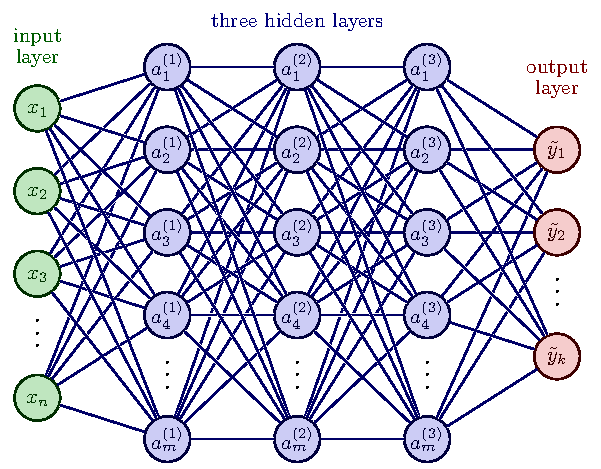
\includegraphics[width=1.0\linewidth]{figures/nn1.pdf}}

\vspace{6mm}

% !split
\subsection{Definitions}

With our definition of the targets $\bm{y}$, the outputs of the
network $\bm{\tilde{y}}$ and the inputs $\bm{x}$ we
define now the activation $z_j^l$ of node/neuron/unit $j$ of the
$l$-th layer as a function of the bias, the weights which add up from
the previous layer $l-1$ and the forward passes/outputs
$\hat{a}^{l-1}$ from the previous layer as

\[
z_j^l = \sum_{i=1}^{M_{l-1}}w_{ij}^la_i^{l-1}+b_j^l,
\]

where $b_k^l$ are the biases from layer $l$.  Here $M_{l-1}$
represents the total number of nodes/neurons/units of layer $l-1$. The
figure in the whiteboard notes illustrates this equation.  We can rewrite this in a more
compact form as the matrix-vector products we discussed earlier,

\[
\hat{z}^l = \left(\hat{W}^l\right)^T\hat{a}^{l-1}+\hat{b}^l.
\]

% !split
\subsection{Inputs to the activation function}

With the activation values $\bm{z}^l$ we can in turn define the
output of layer $l$ as $\bm{a}^l = f(\bm{z}^l)$ where $f$ is our
activation function. In the examples here we will use the sigmoid
function discussed in our logistic regression lectures. We will also use the same activation function $f$ for all layers
and their nodes.  It means we have

\[
a_j^l = \sigma(z_j^l) = \frac{1}{1+\exp{-(z_j^l)}}.
\]

% !split
\subsection{Derivatives and the chain rule}

From the definition of the activation $z_j^l$ we have
\[
\frac{\partial z_j^l}{\partial w_{ij}^l} = a_i^{l-1},
\]
and
\[
\frac{\partial z_j^l}{\partial a_i^{l-1}} = w_{ji}^l. 
\]

With our definition of the activation function we have that (note that this function depends only on $z_j^l$)
\[
\frac{\partial a_j^l}{\partial z_j^{l}} = a_j^l(1-a_j^l)=\sigma(z_j^l)(1-\sigma(z_j^l)). 
\]

% !split
\subsection{Derivative of the cost function}

With these definitions we can now compute the derivative of the cost function in terms of the weights.

Let us specialize to the output layer $l=L$. Our cost function is
\[
{\cal C}(\bm{\Theta}^L)  =  \frac{1}{2}\sum_{i=1}^n\left(y_i - \tilde{y}_i\right)^2=\frac{1}{2}\sum_{i=1}^n\left(a_i^L - y_i\right)^2, 
\]
The derivative of this function with respect to the weights is

\[
\frac{\partial{\cal C}(\bm{\Theta}^L)}{\partial w_{jk}^L}  =  \left(a_j^L - y_j\right)\frac{\partial a_j^L}{\partial w_{jk}^{L}}, 
\]
The last partial derivative can easily be computed and reads (by applying the chain rule)
\[
\frac{\partial a_j^L}{\partial w_{jk}^{L}} = \frac{\partial a_j^L}{\partial z_{j}^{L}}\frac{\partial z_j^L}{\partial w_{jk}^{L}}=a_j^L(1-a_j^L)a_k^{L-1}.  
\]

% !split
\subsection{Simpler examples first, and automatic differentiation}

In order to understand the back propagation algorithm and its
derivation (an implementation of the chain rule), let us first digress
with some simple examples. These examples are also meant to motivate
the link with back propagation and \href{{https://en.wikipedia.org/wiki/Automatic_differentiation}}{automatic differentiation}.

% !split
\subsection{Reminder on the chain rule and gradients}

If we have a multivariate function $f(x,y)$ where $x=x(t)$ and $y=y(t)$ are functions of a variable $t$, we have that the gradient of $f$ with respect to $t$ (without the explicit unit vector components)
\[
\frac{df}{dt} = \begin{bmatrix}\frac{\partial f}{\partial x} & \frac{\partial f}{\partial y} \end{bmatrix} \begin{bmatrix}\frac{\partial x}{\partial t} \\ \frac{\partial y}{\partial t} \end{bmatrix}=\frac{\partial f}{\partial x} \frac{\partial x}{\partial t} +\frac{\partial f}{\partial y} \frac{\partial y}{\partial t}. 
\]

% !split
\subsection{Multivariable functions}

If we have a multivariate function $f(x,y)$ where $x=x(t,s)$ and $y=y(t,s)$ are functions of the variables $t$ and $s$, we have that the partial derivatives
\[
\frac{\partial f}{\partial s}=\frac{\partial f}{\partial x}\frac{\partial x}{\partial s}+\frac{\partial f}{\partial y}\frac{\partial y}{\partial s},
\]
and
\[
\frac{\partial f}{\partial t}=\frac{\partial f}{\partial x}\frac{\partial x}{\partial t}+\frac{\partial f}{\partial y}\frac{\partial y}{\partial t}.
\]

the gradient of $f$ with respect to $t$ and $s$ (without the explicit unit vector components)
\[
\frac{df}{d(s,t)} = \begin{bmatrix}\frac{\partial f}{\partial x} & \frac{\partial f}{\partial y} \end{bmatrix} \begin{bmatrix}\frac{\partial x}{\partial s}  &\frac{\partial x}{\partial t} \\ \frac{\partial y}{\partial s} & \frac{\partial y}{\partial t} \end{bmatrix}.
\]

% !split
\subsection{Automatic differentiation through examples}

A great introduction to automatic differentiation is given by Baydin et al., see \href{{https://arxiv.org/abs/1502.05767}}{\nolinkurl{https://arxiv.org/abs/1502.05767}}.

Automatic differentiation is a represented by a repeated application
of the chain rule on well-known functions and allows for the
calculation of derivatives to numerical precision. It is not the same
as the calculation of symbolic derivatives via for example SymPy, nor
does it use approximative formulae based on Taylor-expansions of a
function around a given value. The latter are error prone due to
truncation errors and values of the step size $\Delta$.

% !split
\subsection{Simple example}

Our first example is rather simple,
\[
f(x) =\exp{x^2},
\]
with derivative
\[
f'(x) =2x\exp{x^2}.
\]
We can use SymPy to extract the pertinent lines of Python code through the following simple example









\bpycod
from __future__ import division
from sympy import *
x = symbols('x')
expr = exp(x*x)
simplify(expr)
derivative = diff(expr,x)
print(python(expr))
print(python(derivative))

\epycod


% !split
\subsection{Smarter way of evaluating the above function}
If we study this function, we note that we can reduce the number of operations by introducing an intermediate variable
\[
a = x^2,
\]
leading to 
\[
f(x) = f(a(x)) = b= \exp{a}.
\]

We now assume that all operations can be counted in terms of equal
floating point operations. This means that in order to calculate
$f(x)$ we need first to square $x$ and then compute the exponential. We
have thus two floating point operations only.

% !split
\subsection{Reducing the number of operations}

With the introduction of a precalculated quantity $a$ and thereby $f(x)$ we have that the derivative can be written as

\[
f'(x) = 2xb,
\]

which reduces the number of operations from four in the orginal
expression to two. This means that if we need to compute $f(x)$ and
its derivative (a common task in optimizations), we have reduced the
number of operations from six to four in total.

\textbf{Note} that the usage of a symbolic software like SymPy does not
include such simplifications and the calculations of the function and
the derivatives yield in general more floating point operations.

% !split
\subsection{Chain rule, forward and reverse modes}

In the above example we have introduced the variables $a$ and $b$, and our function is
\[
f(x) = f(a(x)) = b= \exp{a},
\]
with $a=x^2$. We can decompose the derivative of $f$ with respect to $x$ as
\[
\frac{df}{dx}=\frac{df}{db}\frac{db}{da}\frac{da}{dx}.
\]

We note that since $b=f(x)$ that
\[
\frac{df}{db}=1,
\]
leading to
\[
\frac{df}{dx}=\frac{db}{da}\frac{da}{dx}=2x\exp{x^2},
\]
as before.

% !split
\subsection{Forward and reverse modes}

We have that 
\[
\frac{df}{dx}=\frac{df}{db}\frac{db}{da}\frac{da}{dx},
\]
which we can rewrite either as
\[
\frac{df}{dx}=\left[\frac{df}{db}\frac{db}{da}\right]\frac{da}{dx},
\]
or
\[
\frac{df}{dx}=\frac{df}{db}\left[\frac{db}{da}\frac{da}{dx}\right].
\]

The first expression is called reverse mode (or back propagation)
since we start by evaluating the derivatives at the end point and then
propagate backwards. This is the standard way of evaluating
derivatives (gradients) when optimizing the parameters of a neural
network).  In the context of deep learning this is computationally
more efficient since the output of a neural network consists of either
one or some few other output variables.

The second equation defines the so-called  \textbf{forward mode}.

% !split
\subsection{More complicated function}

We increase our ambitions and introduce a slightly more complicated function
\[
f(x) =\sqrt{x^2+exp{x^2}},
\]
with derivative
\[
f'(x) =\frac{x(1+\exp{x^2})}{\sqrt{x^2+exp{x^2}}}.
\]
The corresponding SymPy code reads









\bpycod
from __future__ import division
from sympy import *
x = symbols('x')
expr = sqrt(x*x+exp(x*x))
simplify(expr)
derivative = diff(expr,x)
print(python(expr))
print(python(derivative))

\epycod


% !split
\subsection{Counting the number of floating point operations}

A simple count of operations shows that we need five operations for
the function itself and ten for the derivative.  Fifteen operations in total if we wish to proceed with the above codes.

Can we reduce this to
say half the number of operations?

% !split
\subsection{Defining intermediate operations}

We can indeed reduce the number of operation to half of those listed in the brute force approach above.
We define the following quantities
\[
a = x^2,
\]
and
\[
b = \exp{x^2} = \exp{a},
\]
and
\[
c= a+b,
\]
and
\[
d=f(x)=\sqrt{c}.
\]

% !split
\subsection{New expression for the derivative}

With these definitions we obtain the following partial derivatives 
\[
\frac{\partial a}{\partial x} = 2x,
\]
and
\[
\frac{\partial b}{\partial a} = \exp{a},
\]
and
\[
\frac{\partial c}{\partial a} = 1,
\]
and
\[
\frac{\partial c}{\partial b} = 1,
\]
and
\[
\frac{\partial d}{\partial c} = \frac{1}{2\srqt{c}},
\]
and finally
\[
\frac{\partial f}{\partial d} = 1.
\]

% !split
\subsection{Final derivatives}
Our final derivatives are thus
\[
\frac{\partial f}{\partial c} = \frac{\partial f}{\partial d} \frac{\partial d}{\partial c}  = \frac{1}{2\srqt{c}},
\]
\[
\frac{\partial f}{\partial b} = \frac{\partial f}{\partial c} \frac{\partial c}{\partial b}  = \frac{1}{2\srqt{c}},
\]
\[
\frac{\partial f}{\partial a} = \frac{\partial f}{\partial c} \frac{\partial c}{\partial a}+
\frac{\partial f}{\partial b} \frac{\partial b}{\partial a}  = \frac{1+\exp{a}}{2\srqt{c}},
\]
and finally 
\[
\frac{\partial f}{\partial x} = \frac{\partial f}{\partial a} \frac{\partial a}{\partial x}  = \frac{x(1+\exp{a})}{\srqt{c}},
\]
which is just
\[
\frac{\partial f}{\partial x} = \frac{x(1+b)}{d},
\]
and requires only three operations if we can reuse all intermediate variables.

% !split
\subsection{First back propagation equation}

We have thus
\[
\frac{\partial{\cal C}((\bm{\Theta}^L)}{\partial w_{jk}^L}  =  \left(a_j^L - y_j\right)a_j^L(1-a_j^L)a_k^{L-1}, 
\]

Defining
\[
\delta_j^L = a_j^L(1-a_j^L)\left(a_j^L - y_j\right) = \sigma'(z_j^L)\frac{\partial {\cal C}}{\partial (a_j^L)},
\]
and using the Hadamard product of two vectors we can write this as
\[
\bm{\delta}^L = \sigma'(\hat{z}^L)\circ\frac{\partial {\cal C}}{\partial (\bm{a}^L)}.
\]

% !split
\subsection{Analyzing the last results}

This is an important expression. The second term on the right handside
measures how fast the cost function is changing as a function of the $j$th
output activation.  If, for example, the cost function doesn't depend
much on a particular output node $j$, then $\delta_j^L$ will be small,
which is what we would expect. The first term on the right, measures
how fast the activation function $f$ is changing at a given activation
value $z_j^L$.

% !split
\subsection{More considerations}

Notice that everything in the above equations is easily computed.  In
particular, we compute $z_j^L$ while computing the behaviour of the
network, and it is only a small additional overhead to compute
$\sigma'(z^L_j)$.  The exact form of the derivative with respect to the
output depends on the form of the cost function.
However, provided the cost function is known there should be little
trouble in calculating

\[
\frac{\partial {\cal C}}{\partial (a_j^L)}
\]

With the definition of $\delta_j^L$ we have a more compact definition of the derivative of the cost function in terms of the weights, namely
\[
\frac{\partial{\cal C}}{\partial w_{jk}^L}  =  \delta_j^La_k^{L-1}.
\]

% !split
\subsection{Derivatives in terms of $z_j^L$}

It is also easy to see that our previous equation can be written as

\[
\delta_j^L =\frac{\partial {\cal C}}{\partial z_j^L}= \frac{\partial {\cal C}}{\partial a_j^L}\frac{\partial a_j^L}{\partial z_j^L},
\]
which can also be interpreted as the partial derivative of the cost function with respect to the biases $b_j^L$, namely
\[
\delta_j^L = \frac{\partial {\cal C}}{\partial b_j^L}\frac{\partial b_j^L}{\partial z_j^L}=\frac{\partial {\cal C}}{\partial b_j^L},
\]
That is, the error $\delta_j^L$ is exactly equal to the rate of change of the cost function as a function of the bias. 

% !split
\subsection{Bringing it together}

We have now three equations that are essential for the computations of the derivatives of the cost function at the output layer. These equations are needed to start the algorithm and they are

\begin{equation}
\frac{\partial{\cal C}(\hat{W^L})}{\partial w_{jk}^L}  =  \delta_j^La_k^{L-1},
\end{equation}
and
\begin{equation}
\delta_j^L = \sigma'(z_j^L)\frac{\partial {\cal C}}{\partial (a_j^L)},
\end{equation}
and

\begin{equation}
\delta_j^L = \frac{\partial {\cal C}}{\partial b_j^L},
\end{equation}

% !split
\subsection{Final back propagating equation}

We have that (replacing $L$ with a general layer $l$)
\[
\delta_j^l =\frac{\partial {\cal C}}{\partial z_j^l}.
\]
We want to express this in terms of the equations for layer $l+1$.

% !split
\subsection{Using the chain rule and summing over all $k$ entries}

We obtain
\[
\delta_j^l =\sum_k \frac{\partial {\cal C}}{\partial z_k^{l+1}}\frac{\partial z_k^{l+1}}{\partial z_j^{l}}=\sum_k \delta_k^{l+1}\frac{\partial z_k^{l+1}}{\partial z_j^{l}},
\]
and recalling that
\[
z_j^{l+1} = \sum_{i=1}^{M_{l}}w_{ij}^{l+1}a_i^{l}+b_j^{l+1},
\]
with $M_l$ being the number of nodes in layer $l$, we obtain
\[
\delta_j^l =\sum_k \delta_k^{l+1}w_{kj}^{l+1}\sigma'(z_j^l),
\]
This is our final equation.

We are now ready to set up the algorithm for back propagation and learning the weights and biases.

% !split
\subsection{Setting up the back propagation algorithm}

The four equations  provide us with a way of computing the gradient of the cost function. Let us write this out in the form of an algorithm.

\textbf{First}, we set up the input data $\hat{x}$ and the activations
$\hat{z}_1$ of the input layer and compute the activation function and
the pertinent outputs $\hat{a}^1$.

\textbf{Secondly}, we perform then the feed forward till we reach the output
layer and compute all $\hat{z}_l$ of the input layer and compute the
activation function and the pertinent outputs $\hat{a}^l$ for
$l=1,2,3,\dots,L$.

\textbf{Notation}: The first hidden layer has $l=1$ as label and the final output layer has $l=L$.

% !split
\subsection{Setting up the back propagation algorithm, part 2}

Thereafter we compute the ouput error $\hat{\delta}^L$ by computing all
\[
\delta_j^L = \sigma'(z_j^L)\frac{\partial {\cal C}}{\partial (a_j^L)}.
\]

Then we compute the back propagate error for each $l=L-1,L-2,\dots,1$ as
\[
\delta_j^l = \sum_k \delta_k^{l+1}w_{kj}^{l+1}\sigma'(z_j^l).
\]

% !split
\subsection{Setting up the Back propagation algorithm, part 3}

Finally, we update the weights and the biases using gradient descent
for each $l=L-1,L-2,\dots,1$ and update the weights and biases
according to the rules

\[
w_{jk}^l\leftarrow  = w_{jk}^l- \eta \delta_j^la_k^{l-1},
\]

\[
b_j^l \leftarrow b_j^l-\eta \frac{\partial {\cal C}}{\partial b_j^l}=b_j^l-\eta \delta_j^l,
\]
with $\eta$ being the learning rate.

% !split
\subsection{Updating the gradients}

With the back propagate error for each $l=L-1,L-2,\dots,1$ as
\[
\delta_j^l = \sum_k \delta_k^{l+1}w_{kj}^{l+1}sigma'(z_j^l),
\]
we update the weights and the biases using gradient descent for each $l=L-1,L-2,\dots,1$ and update the weights and biases according to the rules
\[
w_{jk}^l\leftarrow  = w_{jk}^l- \eta \delta_j^la_k^{l-1},
\]

\[
b_j^l \leftarrow b_j^l-\eta \frac{\partial {\cal C}}{\partial b_j^l}=b_j^l-\eta \delta_j^l,
\]

% !split
\subsection{Fine-tuning neural network hyperparameters}

The flexibility of neural networks is also one of their main
drawbacks: there are many hyperparameters to tweak. Not only can you
use any imaginable network topology (how neurons/nodes are
interconnected), but even in a simple FFNN you can change the number
of layers, the number of neurons per layer, the type of activation
function to use in each layer, the weight initialization logic, the
stochastic gradient optmized and much more. How do you know what
combination of hyperparameters is the best for your task?

\begin{itemize}
\item You can use grid search with cross-validation to find the right hyperparameters.
\end{itemize}

\noindent
However,since there are many hyperparameters to tune, and since
training a neural network on a large dataset takes a lot of time, you
will only be able to explore a tiny part of the hyperparameter space.

\begin{itemize}
\item You can use randomized search.

\item Or use tools like \href{{http://oscar.calldesk.ai/}}{Oscar}, which implements more complex algorithms to help you find a good set of hyperparameters quickly.  
\end{itemize}

\noindent
% !split
\subsection{Hidden layers}

For many problems you can start with just one or two hidden layers and
it will work just fine.  For the MNIST data set you ca easily get a
high accuracy using just one hidden layer with a few hundred neurons.
You can reach for this data set above 98\% accuracy using two hidden
layers with the same total amount of neurons, in roughly the same
amount of training time.

For more complex problems, you can gradually ramp up the number of
hidden layers, until you start overfitting the training set. Very
complex tasks, such as large image classification or speech
recognition, typically require networks with dozens of layers and they
need a huge amount of training data. However, you will rarely have to
train such networks from scratch: it is much more common to reuse
parts of a pretrained state-of-the-art network that performs a similar
task.

% !split 
\subsection{Which activation function should I use?}

The Back propagation algorithm we derived above works by going from
the output layer to the input layer, propagating the error gradient on
the way. Once the algorithm has computed the gradient of the cost
function with regards to each parameter in the network, it uses these
gradients to update each parameter with a Gradient Descent (GD) step.

Unfortunately for us, the gradients often get smaller and smaller as
the algorithm progresses down to the first hidden layers. As a result,
the GD update leaves the lower layer connection weights virtually
unchanged, and training never converges to a good solution. This is
known in the literature as \textbf{the vanishing gradients problem}.

In other cases, the opposite can happen, namely the the gradients can
grow bigger and bigger. The result is that many of the layers get
large updates of the weights the algorithm diverges. This is the
\textbf{exploding gradients problem}, which is mostly encountered in
recurrent neural networks. More generally, deep neural networks suffer
from unstable gradients, different layers may learn at widely
different speeds

% !split 
\subsection{Is the Logistic activation function (Sigmoid)  our choice?}

Although this unfortunate behavior has been empirically observed for
quite a while (it was one of the reasons why deep neural networks were
mostly abandoned for a long time), it is only around 2010 that
significant progress was made in understanding it.

A paper titled \href{{http://proceedings.mlr.press/v9/glorot10a.html}}{Understanding the Difficulty of Training Deep
Feedforward Neural Networks by Xavier Glorot and Yoshua Bengio} found that
the problems with the popular logistic
sigmoid activation function and the weight initialization technique
that was most popular at the time, namely random initialization using
a normal distribution with a mean of 0 and a standard deviation of
1. 

They showed that with this activation function and this
initialization scheme, the variance of the outputs of each layer is
much greater than the variance of its inputs. Going forward in the
network, the variance keeps increasing after each layer until the
activation function saturates at the top layers. This is actually made
worse by the fact that the logistic function has a mean of 0.5, not 0
(the hyperbolic tangent function has a mean of 0 and behaves slightly
better than the logistic function in deep networks).

% !split
\subsection{The derivative of the Logistic funtion}

Looking at the logistic activation function, when inputs become large
(negative or positive), the function saturates at 0 or 1, with a
derivative extremely close to 0. Thus when backpropagation kicks in,
it has virtually no gradient to propagate back through the network,
and what little gradient exists keeps getting diluted as
backpropagation progresses down through the top layers, so there is
really nothing left for the lower layers.

In their paper, Glorot and Bengio propose a way to significantly
alleviate this problem. We need the signal to flow properly in both
directions: in the forward direction when making predictions, and in
the reverse direction when backpropagating gradients. We don’t want
the signal to die out, nor do we want it to explode and saturate. For
the signal to flow properly, the authors argue that we need the
variance of the outputs of each layer to be equal to the variance of
its inputs, and we also need the gradients to have equal variance
before and after flowing through a layer in the reverse direction.

% !split
\subsection{Insights from the paper by Glorot and Bengio}

One of the insights in the 2010 paper by Glorot and Bengio was that
the vanishing/exploding gradients problems were in part due to a poor
choice of activation function. Until then most people had assumed that
if Nature had chosen to use roughly sigmoid activation functions in
biological neurons, they must be an excellent choice. But it turns out
that other activation functions behave much better in deep neural
networks, in particular the ReLU activation function, mostly because
it does not saturate for positive values (and also because it is quite
fast to compute).

% !split
\subsection{The RELU function family}

The ReLU activation function suffers from a problem known as the dying
ReLUs: during training, some neurons effectively die, meaning they
stop outputting anything other than 0.

In some cases, you may find that half of your network’s neurons are
dead, especially if you used a large learning rate. During training,
if a neuron’s weights get updated such that the weighted sum of the
neuron’s inputs is negative, it will start outputting 0. When this
happen, the neuron is unlikely to come back to life since the gradient
of the ReLU function is 0 when its input is negative.

To solve this problem, nowadays practitioners use a variant of the
ReLU function, such as the leaky ReLU discussed above or the so-called
exponential linear unit (ELU) function

\[
ELU(z) = \left\{\begin{array}{cc} \alpha\left( \exp{(z)}-1\right) & z < 0,\\  z & z \ge 0.\end{array}\right. 
\]

% !split
\subsection{Which activation function should we use?}

In general it seems that the ELU activation function is better than
the leaky ReLU function (and its variants), which is better than
ReLU. ReLU performs better than $\tanh$ which in turn performs better
than the logistic function.

If runtime performance is an issue, then you may opt for the leaky
ReLU function over the ELU function If you don’t want to tweak yet
another hyperparameter, you may just use the default $\alpha$ of
$0.01$ for the leaky ReLU, and $1$ for ELU. If you have spare time and
computing power, you can use cross-validation or bootstrap to evaluate
other activation functions.

% !split
\subsection{More on activation functions, output layers}

In most cases you can use the ReLU activation function in the hidden
layers (or one of its variants).

It is a bit faster to compute than other activation functions, and the
gradient descent optimization does in general not get stuck.

\textbf{For the output layer:}

\begin{itemize}
\item For classification the softmax activation function is generally a good choice for classification tasks (when the classes are mutually exclusive).

\item For regression tasks, you can simply use no activation function at all.
\end{itemize}

\noindent
% !split
\subsection{Batch Normalization}

Batch Normalization aims to address the vanishing/exploding gradients
problems, and more generally the problem that the distribution of each
layer’s inputs changes during training, as the parameters of the
previous layers change.

The technique consists of adding an operation in the model just before
the activation function of each layer, simply zero-centering and
normalizing the inputs, then scaling and shifting the result using two
new parameters per layer (one for scaling, the other for shifting). In
other words, this operation lets the model learn the optimal scale and
mean of the inputs for each layer.  In order to zero-center and
normalize the inputs, the algorithm needs to estimate the inputs’ mean
and standard deviation. It does so by evaluating the mean and standard
deviation of the inputs over the current mini-batch, from this the
name batch normalization.

% !split
\subsection{Dropout}

It is a fairly simple algorithm: at every training step, every neuron
(including the input neurons but excluding the output neurons) has a
probability $p$ of being temporarily dropped out, meaning it will be
entirely ignored during this training step, but it may be active
during the next step.

The hyperparameter $p$ is called the dropout rate, and it is typically
set to 50\%. After training, the neurons are not dropped anymore.  It
is viewed as one of the most popular regularization techniques.

% !split
\subsection{Gradient Clipping}

A popular technique to lessen the exploding gradients problem is to
simply clip the gradients during backpropagation so that they never
exceed some threshold (this is mostly useful for recurrent neural
networks).

This technique is called Gradient Clipping.

In general however, Batch
Normalization is preferred.

% !split 
\subsection{A top-down perspective on Neural networks}

The first thing we would like to do is divide the data into two or
three parts. A training set, a validation or dev (development) set,
and a test set. The test set is the data on which we want to make
predictions. The dev set is a subset of the training data we use to
check how well we are doing out-of-sample, after training the model on
the training dataset. We use the validation error as a proxy for the
test error in order to make tweaks to our model. It is crucial that we
do not use any of the test data to train the algorithm. This is a
cardinal sin in ML. Then:

\begin{itemize}
\item Estimate optimal error rate

\item Minimize underfitting (bias) on training data set.

\item Make sure you are not overfitting.
\end{itemize}

\noindent
% !split
\subsection{More top-down perspectives}

If the validation and test sets are drawn from the same distributions,
then a good performance on the validation set should lead to similarly
good performance on the test set. 

However, sometimes
the training data and test data differ in subtle ways because, for
example, they are collected using slightly different methods, or
because it is cheaper to collect data in one way versus another. In
this case, there can be a mismatch between the training and test
data. This can lead to the neural network overfitting these small
differences between the test and training sets, and a poor performance
on the test set despite having a good performance on the validation
set. To rectify this, Andrew Ng suggests making two validation or dev
sets, one constructed from the training data and one constructed from
the test data. The difference between the performance of the algorithm
on these two validation sets quantifies the train-test mismatch. This
can serve as another important diagnostic when using DNNs for
supervised learning.

% !split
\subsection{Limitations of supervised learning with deep networks}

Like all statistical methods, supervised learning using neural
networks has important limitations. This is especially important when
one seeks to apply these methods, especially to physics problems. Like
all tools, DNNs are not a universal solution. Often, the same or
better performance on a task can be achieved by using a few
hand-engineered features (or even a collection of random
features). 

% !split
\subsection{Limitations of NNs}

Here we list some of the important limitations of supervised neural network based models. 

\begin{itemize}
\item \textbf{Need labeled data}. All supervised learning methods, DNNs for supervised learning require labeled data. Often, labeled data is harder to acquire than unlabeled data (e.g.~one must pay for human experts to label images).

\item \textbf{Supervised neural networks are extremely data intensive.} DNNs are data hungry. They perform best when data is plentiful. This is doubly so for supervised methods where the data must also be labeled. The utility of DNNs is extremely limited if data is hard to acquire or the datasets are small (hundreds to a few thousand samples). In this case, the performance of other methods that utilize hand-engineered features can exceed that of DNNs.
\end{itemize}

\noindent
% !split
\subsection{Homogeneous data}

\begin{itemize}
\item \textbf{Homogeneous data.} Almost all DNNs deal with homogeneous data of one type. It is very hard to design architectures that mix and match data types (i.e.~some continuous variables, some discrete variables, some time series). In applications beyond images, video, and language, this is often what is required. In contrast, ensemble models like random forests or gradient-boosted trees have no difficulty handling mixed data types.
\end{itemize}

\noindent
% !split
\subsection{More limitations}

\begin{itemize}
\item \textbf{Many problems are not about prediction.} In natural science we are often interested in learning something about the underlying distribution that generates the data. In this case, it is often difficult to cast these ideas in a supervised learning setting. While the problems are related, it is possible to make good predictions with a \emph{wrong} model. The model might or might not be useful for understanding the underlying science.
\end{itemize}

\noindent
Some of these remarks are particular to DNNs, others are shared by all supervised learning methods. This motivates the use of unsupervised methods which in part circumvent these problems.

% !split
\subsection{Building a neural network code}

Here we  present a flexible object oriented codebase
for a feed forward neural network, along with a demonstration of how
to use it. Before we get into the details of the neural network, we
will first present some implementations of various schedulers, cost
functions and activation functions that can be used together with the
neural network.

The codes here were developed by Eric Reber and Gregor Kajda during spring 2023.
After these codes we present the TensorFlow inplementation. Pytorch will be discussed next week.

% !split
\subsection{Learning rate methods}

The code below shows object oriented implementations of the Constant,
Momentum, Adagrad, AdagradMomentum, RMS prop and Adam schedulers. All
of the classes belong to the shared abstract \textbf{Scheduler class}, and
share the update$\_$change() and reset() methods allowing for any of the
schedulers to be seamlessly used during the training stage, as will
later be shown in the fit() method of the neural
network. Update$\_$change() only has one parameter, the gradient, and returns the change which will be subtracted
from the weights. The reset() function takes no parameters, and resets
the desired variables. For Constant and Momentum, reset does nothing.





































































































































\bpycod
import autograd.numpy as np

class Scheduler:
    """
    Abstract class for Schedulers
    """

    def __init__(self, eta):
        self.eta = eta

    # should be overwritten
    def update_change(self, gradient):
        raise NotImplementedError

    # overwritten if needed
    def reset(self):
        pass


class Constant(Scheduler):
    def __init__(self, eta):
        super().__init__(eta)

    def update_change(self, gradient):
        return self.eta * gradient
    
    def reset(self):
        pass


class Momentum(Scheduler):
    def __init__(self, eta: float, momentum: float):
        super().__init__(eta)
        self.momentum = momentum
        self.change = 0

    def update_change(self, gradient):
        self.change = self.momentum * self.change + self.eta * gradient
        return self.change

    def reset(self):
        pass


class Adagrad(Scheduler):
    def __init__(self, eta):
        super().__init__(eta)
        self.G_t = None

    def update_change(self, gradient):
        delta = 1e-8  # avoid division ny zero

        if self.G_t is None:
            self.G_t = np.zeros((gradient.shape[0], gradient.shape[0]))

        self.G_t += gradient @ gradient.T

        G_t_inverse = 1 / (
            delta + np.sqrt(np.reshape(np.diagonal(self.G_t), (self.G_t.shape[0], 1)))
        )
        return self.eta * gradient * G_t_inverse

    def reset(self):
        self.G_t = None


class AdagradMomentum(Scheduler):
    def __init__(self, eta, momentum):
        super().__init__(eta)
        self.G_t = None
        self.momentum = momentum
        self.change = 0

    def update_change(self, gradient):
        delta = 1e-8  # avoid division ny zero

        if self.G_t is None:
            self.G_t = np.zeros((gradient.shape[0], gradient.shape[0]))

        self.G_t += gradient @ gradient.T

        G_t_inverse = 1 / (
            delta + np.sqrt(np.reshape(np.diagonal(self.G_t), (self.G_t.shape[0], 1)))
        )
        self.change = self.change * self.momentum + self.eta * gradient * G_t_inverse
        return self.change

    def reset(self):
        self.G_t = None


class RMS_prop(Scheduler):
    def __init__(self, eta, rho):
        super().__init__(eta)
        self.rho = rho
        self.second = 0.0

    def update_change(self, gradient):
        delta = 1e-8  # avoid division ny zero
        self.second = self.rho * self.second + (1 - self.rho) * gradient * gradient
        return self.eta * gradient / (np.sqrt(self.second + delta))

    def reset(self):
        self.second = 0.0


class Adam(Scheduler):
    def __init__(self, eta, rho, rho2):
        super().__init__(eta)
        self.rho = rho
        self.rho2 = rho2
        self.moment = 0
        self.second = 0
        self.n_epochs = 1

    def update_change(self, gradient):
        delta = 1e-8  # avoid division ny zero

        self.moment = self.rho * self.moment + (1 - self.rho) * gradient
        self.second = self.rho2 * self.second + (1 - self.rho2) * gradient * gradient

        moment_corrected = self.moment / (1 - self.rho**self.n_epochs)
        second_corrected = self.second / (1 - self.rho2**self.n_epochs)

        return self.eta * moment_corrected / (np.sqrt(second_corrected + delta))

    def reset(self):
        self.n_epochs += 1
        self.moment = 0
        self.second = 0


\epycod


% !split
\subsection{Usage of the above learning rate schedulers}

To initalize a scheduler, simply create the object and pass in the
necessary parameters such as the learning rate and the momentum as
shown below. As the Scheduler class is an abstract class it should not
called directly, and will raise an error upon usage.




\bpycod
momentum_scheduler = Momentum(eta=1e-3, momentum=0.9)
adam_scheduler = Adam(eta=1e-3, rho=0.9, rho2=0.999)

\epycod


Here is a small example for how a segment of code using schedulers
could look. Switching out the schedulers is simple.













\bpycod
weights = np.ones((3,3))
print(f"Before scheduler:\n{weights=}")

epochs = 10
for e in range(epochs):
    gradient = np.random.rand(3, 3)
    change = adam_scheduler.update_change(gradient)
    weights = weights - change
    adam_scheduler.reset()

print(f"\nAfter scheduler:\n{weights=}")

\epycod


% !split
\subsection{Cost functions}

Here we discuss cost functions that can be used when creating the
neural network. Every cost function takes the target vector as its
parameter, and returns a function valued only at $x$ such that it may
easily be differentiated.





























\bpycod
import autograd.numpy as np

def CostOLS(target):
    
    def func(X):
        return (1.0 / target.shape[0]) * np.sum((target - X) ** 2)

    return func


def CostLogReg(target):

    def func(X):
        
        return -(1.0 / target.shape[0]) * np.sum(
            (target * np.log(X + 10e-10)) + ((1 - target) * np.log(1 - X + 10e-10))
        )

    return func


def CostCrossEntropy(target):
    
    def func(X):
        return -(1.0 / target.size) * np.sum(target * np.log(X + 10e-10))

    return func

\epycod


Below we give a short example of how these cost function may be used
to obtain results if you wish to test them out on your own using
AutoGrad's automatics differentiation.












\bpycod
from autograd import grad

target = np.array([[1, 2, 3]]).T
a = np.array([[4, 5, 6]]).T

cost_func = CostCrossEntropy
cost_func_derivative = grad(cost_func(target))

valued_at_a = cost_func_derivative(a)
print(f"Derivative of cost function {cost_func.__name__} valued at a:\n{valued_at_a}")

\epycod


% !split
\subsection{Activation functions}

Finally, before we look at the neural network, we will look at the
activation functions which can be specified between the hidden layers
and as the output function. Each function can be valued for any given
vector or matrix X, and can be differentiated via derivate().

















































\bpycod
import autograd.numpy as np
from autograd import elementwise_grad

def identity(X):
    return X


def sigmoid(X):
    try:
        return 1.0 / (1 + np.exp(-X))
    except FloatingPointError:
        return np.where(X > np.zeros(X.shape), np.ones(X.shape), np.zeros(X.shape))


def softmax(X):
    X = X - np.max(X, axis=-1, keepdims=True)
    delta = 10e-10
    return np.exp(X) / (np.sum(np.exp(X), axis=-1, keepdims=True) + delta)


def RELU(X):
    return np.where(X > np.zeros(X.shape), X, np.zeros(X.shape))


def LRELU(X):
    delta = 10e-4
    return np.where(X > np.zeros(X.shape), X, delta * X)


def derivate(func):
    if func.__name__ == "RELU":

        def func(X):
            return np.where(X > 0, 1, 0)

        return func

    elif func.__name__ == "LRELU":

        def func(X):
            delta = 10e-4
            return np.where(X > 0, 1, delta)

        return func

    else:
        return elementwise_grad(func)

\epycod


Below follows a short demonstration of how to use an activation
function. The derivative of the activation function will be important
when calculating the output delta term during backpropagation. Note
that derivate() can also be used for cost functions for a more
generalized approach.












\bpycod
z = np.array([[4, 5, 6]]).T
print(f"Input to activation function:\n{z}")

act_func = sigmoid
a = act_func(z)
print(f"\nOutput from {act_func.__name__} activation function:\n{a}")

act_func_derivative = derivate(act_func)
valued_at_z = act_func_derivative(a)
print(f"\nDerivative of {act_func.__name__} activation function valued at z:\n{valued_at_z}")

\epycod


% !split
\subsection{The Neural Network}

Now that we have gotten a good understanding of the implementation of
some important components, we can take a look at an object oriented
implementation of a feed forward neural network. The feed forward
neural network has been implemented as a class named FFNN, which can
be initiated as a regressor or classifier dependant on the choice of
cost function. The FFNN can have any number of input nodes, hidden
layers with any amount of hidden nodes, and any amount of output nodes
meaning it can perform multiclass classification as well as binary
classification and regression problems. Although there is a lot of
code present, it makes for an easy to use and generalizeable interface
for creating many types of neural networks as will be demonstrated
below.















































































































































































































































































































































































































































































\bpycod
import math
import autograd.numpy as np
import sys
import warnings
from autograd import grad, elementwise_grad
from random import random, seed
from copy import deepcopy, copy
from typing import Tuple, Callable
from sklearn.utils import resample

warnings.simplefilter("error")


class FFNN:
    """
    Description:
    ------------
        Feed Forward Neural Network with interface enabling flexible design of a
        nerual networks architecture and the specification of activation function
        in the hidden layers and output layer respectively. This model can be used
        for both regression and classification problems, depending on the output function.

    Attributes:
    ------------
        I   dimensions (tuple[int]): A list of positive integers, which specifies the
            number of nodes in each of the networks layers. The first integer in the array
            defines the number of nodes in the input layer, the second integer defines number
            of nodes in the first hidden layer and so on until the last number, which
            specifies the number of nodes in the output layer.
        II  hidden_func (Callable): The activation function for the hidden layers
        III output_func (Callable): The activation function for the output layer
        IV  cost_func (Callable): Our cost function
        V   seed (int): Sets random seed, makes results reproducible
    """

    def __init__(
        self,
        dimensions: tuple[int],
        hidden_func: Callable = sigmoid,
        output_func: Callable = lambda x: x,
        cost_func: Callable = CostOLS,
        seed: int = None,
    ):
        self.dimensions = dimensions
        self.hidden_func = hidden_func
        self.output_func = output_func
        self.cost_func = cost_func
        self.seed = seed
        self.weights = list()
        self.schedulers_weight = list()
        self.schedulers_bias = list()
        self.a_matrices = list()
        self.z_matrices = list()
        self.classification = None

        self.reset_weights()
        self._set_classification()

    def fit(
        self,
        X: np.ndarray,
        t: np.ndarray,
        scheduler: Scheduler,
        batches: int = 1,
        epochs: int = 100,
        lam: float = 0,
        X_val: np.ndarray = None,
        t_val: np.ndarray = None,
    ):
        """
        Description:
        ------------
            This function performs the training the neural network by performing the feedforward and backpropagation
            algorithm to update the networks weights.

        Parameters:
        ------------
            I    X (np.ndarray) : training data
            II   t (np.ndarray) : target data
            III  scheduler (Scheduler) : specified scheduler (algorithm for optimization of gradient descent)
            IV   scheduler_args (list[int]) : list of all arguments necessary for scheduler

        Optional Parameters:
        ------------
            V    batches (int) : number of batches the datasets are split into, default equal to 1
            VI   epochs (int) : number of iterations used to train the network, default equal to 100
            VII  lam (float) : regularization hyperparameter lambda
            VIII X_val (np.ndarray) : validation set
            IX   t_val (np.ndarray) : validation target set

        Returns:
        ------------
            I   scores (dict) : A dictionary containing the performance metrics of the model.
                The number of the metrics depends on the parameters passed to the fit-function.

        """

        # setup 
        if self.seed is not None:
            np.random.seed(self.seed)

        val_set = False
        if X_val is not None and t_val is not None:
            val_set = True

        # creating arrays for score metrics
        train_errors = np.empty(epochs)
        train_errors.fill(np.nan)
        val_errors = np.empty(epochs)
        val_errors.fill(np.nan)

        train_accs = np.empty(epochs)
        train_accs.fill(np.nan)
        val_accs = np.empty(epochs)
        val_accs.fill(np.nan)

        self.schedulers_weight = list()
        self.schedulers_bias = list()

        batch_size = X.shape[0] // batches

        X, t = resample(X, t)

        # this function returns a function valued only at X
        cost_function_train = self.cost_func(t)
        if val_set:
            cost_function_val = self.cost_func(t_val)

        # create schedulers for each weight matrix
        for i in range(len(self.weights)):
            self.schedulers_weight.append(copy(scheduler))
            self.schedulers_bias.append(copy(scheduler))

        print(f"{scheduler.__class__.__name__}: Eta={scheduler.eta}, Lambda={lam}")

        try:
            for e in range(epochs):
                for i in range(batches):
                    # allows for minibatch gradient descent
                    if i == batches - 1:
                        # If the for loop has reached the last batch, take all thats left
                        X_batch = X[i * batch_size :, :]
                        t_batch = t[i * batch_size :, :]
                    else:
                        X_batch = X[i * batch_size : (i + 1) * batch_size, :]
                        t_batch = t[i * batch_size : (i + 1) * batch_size, :]

                    self._feedforward(X_batch)
                    self._backpropagate(X_batch, t_batch, lam)

                # reset schedulers for each epoch (some schedulers pass in this call)
                for scheduler in self.schedulers_weight:
                    scheduler.reset()

                for scheduler in self.schedulers_bias:
                    scheduler.reset()

                # computing performance metrics
                pred_train = self.predict(X)
                train_error = cost_function_train(pred_train)

                train_errors[e] = train_error
                if val_set:
                    
                    pred_val = self.predict(X_val)
                    val_error = cost_function_val(pred_val)
                    val_errors[e] = val_error

                if self.classification:
                    train_acc = self._accuracy(self.predict(X), t)
                    train_accs[e] = train_acc
                    if val_set:
                        val_acc = self._accuracy(pred_val, t_val)
                        val_accs[e] = val_acc

                # printing progress bar
                progression = e / epochs
                print_length = self._progress_bar(
                    progression,
                    train_error=train_errors[e],
                    train_acc=train_accs[e],
                    val_error=val_errors[e],
                    val_acc=val_accs[e],
                )
        except KeyboardInterrupt:
            # allows for stopping training at any point and seeing the result
            pass

        # visualization of training progression (similiar to tensorflow progression bar)
        sys.stdout.write("\r" + " " * print_length)
        sys.stdout.flush()
        self._progress_bar(
            1,
            train_error=train_errors[e],
            train_acc=train_accs[e],
            val_error=val_errors[e],
            val_acc=val_accs[e],
        )
        sys.stdout.write("")

        # return performance metrics for the entire run
        scores = dict()

        scores["train_errors"] = train_errors

        if val_set:
            scores["val_errors"] = val_errors

        if self.classification:
            scores["train_accs"] = train_accs

            if val_set:
                scores["val_accs"] = val_accs

        return scores

    def predict(self, X: np.ndarray, *, threshold=0.5):
        """
         Description:
         ------------
             Performs prediction after training of the network has been finished.

         Parameters:
        ------------
             I   X (np.ndarray): The design matrix, with n rows of p features each

         Optional Parameters:
         ------------
             II  threshold (float) : sets minimal value for a prediction to be predicted as the positive class
                 in classification problems

         Returns:
         ------------
             I   z (np.ndarray): A prediction vector (row) for each row in our design matrix
                 This vector is thresholded if regression=False, meaning that classification results
                 in a vector of 1s and 0s, while regressions in an array of decimal numbers

        """

        predict = self._feedforward(X)

        if self.classification:
            return np.where(predict > threshold, 1, 0)
        else:
            return predict

    def reset_weights(self):
        """
        Description:
        ------------
            Resets/Reinitializes the weights in order to train the network for a new problem.

        """
        if self.seed is not None:
            np.random.seed(self.seed)

        self.weights = list()
        for i in range(len(self.dimensions) - 1):
            weight_array = np.random.randn(
                self.dimensions[i] + 1, self.dimensions[i + 1]
            )
            weight_array[0, :] = np.random.randn(self.dimensions[i + 1]) * 0.01

            self.weights.append(weight_array)

    def _feedforward(self, X: np.ndarray):
        """
        Description:
        ------------
            Calculates the activation of each layer starting at the input and ending at the output.
            Each following activation is calculated from a weighted sum of each of the preceeding
            activations (except in the case of the input layer).

        Parameters:
        ------------
            I   X (np.ndarray): The design matrix, with n rows of p features each

        Returns:
        ------------
            I   z (np.ndarray): A prediction vector (row) for each row in our design matrix
        """

        # reset matrices
        self.a_matrices = list()
        self.z_matrices = list()

        # if X is just a vector, make it into a matrix
        if len(X.shape) == 1:
            X = X.reshape((1, X.shape[0]))

        # Add a coloumn of zeros as the first coloumn of the design matrix, in order
        # to add bias to our data
        bias = np.ones((X.shape[0], 1)) * 0.01
        X = np.hstack([bias, X])

        # a^0, the nodes in the input layer (one a^0 for each row in X - where the
        # exponent indicates layer number).
        a = X
        self.a_matrices.append(a)
        self.z_matrices.append(a)

        # The feed forward algorithm
        for i in range(len(self.weights)):
            if i < len(self.weights) - 1:
                z = a @ self.weights[i]
                self.z_matrices.append(z)
                a = self.hidden_func(z)
                # bias column again added to the data here
                bias = np.ones((a.shape[0], 1)) * 0.01
                a = np.hstack([bias, a])
                self.a_matrices.append(a)
            else:
                try:
                    # a^L, the nodes in our output layers
                    z = a @ self.weights[i]
                    a = self.output_func(z)
                    self.a_matrices.append(a)
                    self.z_matrices.append(z)
                except Exception as OverflowError:
                    print(
                        "OverflowError in fit() in FFNN\nHOW TO DEBUG ERROR: Consider lowering your learning rate or scheduler specific parameters such as momentum, or check if your input values need scaling"
                    )

        # this will be a^L
        return a

    def _backpropagate(self, X, t, lam):
        """
        Description:
        ------------
            Performs the backpropagation algorithm. In other words, this method
            calculates the gradient of all the layers starting at the
            output layer, and moving from right to left accumulates the gradient until
            the input layer is reached. Each layers respective weights are updated while
            the algorithm propagates backwards from the output layer (auto-differentation in reverse mode).

        Parameters:
        ------------
            I   X (np.ndarray): The design matrix, with n rows of p features each.
            II  t (np.ndarray): The target vector, with n rows of p targets.
            III lam (float32): regularization parameter used to punish the weights in case of overfitting

        Returns:
        ------------
            No return value.

        """
        out_derivative = derivate(self.output_func)
        hidden_derivative = derivate(self.hidden_func)

        for i in range(len(self.weights) - 1, -1, -1):
            # delta terms for output
            if i == len(self.weights) - 1:
                # for multi-class classification
                if (
                    self.output_func.__name__ == "softmax"
                ):
                    delta_matrix = self.a_matrices[i + 1] - t
                # for single class classification
                else:
                    cost_func_derivative = grad(self.cost_func(t))
                    delta_matrix = out_derivative(
                        self.z_matrices[i + 1]
                    ) * cost_func_derivative(self.a_matrices[i + 1])

            # delta terms for hidden layer
            else:
                delta_matrix = (
                    self.weights[i + 1][1:, :] @ delta_matrix.T
                ).T * hidden_derivative(self.z_matrices[i + 1])

            # calculate gradient
            gradient_weights = self.a_matrices[i][:, 1:].T @ delta_matrix
            gradient_bias = np.sum(delta_matrix, axis=0).reshape(
                1, delta_matrix.shape[1]
            )

            # regularization term
            gradient_weights += self.weights[i][1:, :] * lam

            # use scheduler
            update_matrix = np.vstack(
                [
                    self.schedulers_bias[i].update_change(gradient_bias),
                    self.schedulers_weight[i].update_change(gradient_weights),
                ]
            )

            # update weights and bias
            self.weights[i] -= update_matrix

    def _accuracy(self, prediction: np.ndarray, target: np.ndarray):
        """
        Description:
        ------------
            Calculates accuracy of given prediction to target

        Parameters:
        ------------
            I   prediction (np.ndarray): vector of predicitons output network
                (1s and 0s in case of classification, and real numbers in case of regression)
            II  target (np.ndarray): vector of true values (What the network ideally should predict)

        Returns:
        ------------
            A floating point number representing the percentage of correctly classified instances.
        """
        assert prediction.size == target.size
        return np.average((target == prediction))
    def _set_classification(self):
        """
        Description:
        ------------
            Decides if FFNN acts as classifier (True) og regressor (False),
            sets self.classification during init()
        """
        self.classification = False
        if (
            self.cost_func.__name__ == "CostLogReg"
            or self.cost_func.__name__ == "CostCrossEntropy"
        ):
            self.classification = True

    def _progress_bar(self, progression, **kwargs):
        """
        Description:
        ------------
            Displays progress of training
        """
        print_length = 40
        num_equals = int(progression * print_length)
        num_not = print_length - num_equals
        arrow = ">" if num_equals > 0 else ""
        bar = "[" + "=" * (num_equals - 1) + arrow + "-" * num_not + "]"
        perc_print = self._format(progression * 100, decimals=5)
        line = f"  {bar} {perc_print}% "

        for key in kwargs:
            if not np.isnan(kwargs[key]):
                value = self._format(kwargs[key], decimals=4)
                line += f"| {key}: {value} "
        sys.stdout.write("\r" + line)
        sys.stdout.flush()
        return len(line)

    def _format(self, value, decimals=4):
        """
        Description:
        ------------
            Formats decimal numbers for progress bar
        """
        if value > 0:
            v = value
        elif value < 0:
            v = -10 * value
        else:
            v = 1
        n = 1 + math.floor(math.log10(v))
        if n >= decimals - 1:
            return str(round(value))
        return f"{value:.{decimals-n-1}f}"

\epycod


Before we make a model, we will quickly generate a dataset we can use
for our linear regression problem as shown below




































\bpycod
import autograd.numpy as np
from sklearn.model_selection import train_test_split

def SkrankeFunction(x, y):
    return np.ravel(0 + 1*x + 2*y + 3*x**2 + 4*x*y + 5*y**2)

def create_X(x, y, n):
    if len(x.shape) > 1:
        x = np.ravel(x)
        y = np.ravel(y)

    N = len(x)
    l = int((n + 1) * (n + 2) / 2)  # Number of elements in beta
    X = np.ones((N, l))

    for i in range(1, n + 1):
        q = int((i) * (i + 1) / 2)
        for k in range(i + 1):
            X[:, q + k] = (x ** (i - k)) * (y**k)

    return X

step=0.5
x = np.arange(0, 1, step)
y = np.arange(0, 1, step)
x, y = np.meshgrid(x, y)
target = SkrankeFunction(x, y)
target = target.reshape(target.shape[0], 1)

poly_degree=3
X = create_X(x, y, poly_degree)

X_train, X_test, t_train, t_test = train_test_split(X, target)


\epycod


Now that we have our dataset ready for the regression, we can create
our regressor. Note that with the seed parameter, we can make sure our
results stay the same every time we run the neural network. For
inititialization, we simply specify the dimensions (we wish the amount
of input nodes to be equal to the datapoints, and the output to
predict one value).







\bpycod
input_nodes = X_train.shape[1]
output_nodes = 1

linear_regression = FFNN((input_nodes, output_nodes), output_func=identity, cost_func=CostOLS, seed=2023)


\epycod


We then fit our model with our training data using the scheduler of our choice.








\bpycod
linear_regression.reset_weights() # reset weights such that previous runs or reruns don't affect the weights

scheduler = Constant(eta=1e-3)
scores = linear_regression.fit(X_train, t_train, scheduler)



\epycod


Due to the progress bar we can see the MSE (train$\_$error) throughout
the FFNN's training. Note that the fit() function has some optional
parameters with defualt arguments. For example, the regularization
hyperparameter can be left ignored if not needed, and equally the FFNN
will by default run for 100 epochs. These can easily be changed, such
as for example:






\bpycod
linear_regression.reset_weights() # reset weights such that previous runs or reruns don't affect the weights

scores = linear_regression.fit(X_train, t_train, scheduler, lam=1e-4, epochs=1000)


\epycod


We see that given more epochs to train on, the regressor reaches a lower MSE.

Let us then switch to a binary classification. We use a binary
classification dataset, and follow a similar setup to the regression
case.


















\bpycod
from sklearn.datasets import load_breast_cancer
from sklearn.preprocessing import MinMaxScaler

wisconsin = load_breast_cancer()
X = wisconsin.data
target = wisconsin.target
target = target.reshape(target.shape[0], 1)

X_train, X_val, t_train, t_val = train_test_split(X, target)

scaler = MinMaxScaler()
scaler.fit(X_train)
X_train = scaler.transform(X_train)
X_val = scaler.transform(X_val)



\epycod








\bpycod
input_nodes = X_train.shape[1]
output_nodes = 1

logistic_regression = FFNN((input_nodes, output_nodes), output_func=sigmoid, cost_func=CostLogReg, seed=2023)


\epycod


We will now make use of our validation data by passing it into our fit function as a keyword argument








\bpycod
logistic_regression.reset_weights() # reset weights such that previous runs or reruns don't affect the weights

scheduler = Adam(eta=1e-3, rho=0.9, rho2=0.999)
scores = logistic_regression.fit(X_train, t_train, scheduler, epochs=1000, X_val=X_val, t_val=t_val)



\epycod


Finally, we will create a neural network with 2 hidden layers with activation functions.











\bpycod
input_nodes = X_train.shape[1]
hidden_nodes1 = 100
hidden_nodes2 = 30
output_nodes = 1

dims = (input_nodes, hidden_nodes1, hidden_nodes2, output_nodes)

neural_network = FFNN(dims, hidden_func=RELU, output_func=sigmoid, cost_func=CostLogReg, seed=2023)



\epycod








\bpycod
neural_network.reset_weights() # reset weights such that previous runs or reruns don't affect the weights

scheduler = Adam(eta=1e-4, rho=0.9, rho2=0.999)
scores = neural_network.fit(X_train, t_train, scheduler, epochs=1000, X_val=X_val, t_val=t_val)


\epycod


% !split
\subsection{Multiclass classification}

Finally, we will demonstrate the use case of multiclass classification
using our FFNN with the famous MNIST dataset, which contain images of
digits between the range of 0 to 9.





























\bpycod
from sklearn.datasets import load_digits

def onehot(target: np.ndarray):
    onehot = np.zeros((target.size, target.max() + 1))
    onehot[np.arange(target.size), target] = 1
    return onehot

digits = load_digits()

X = digits.data
target = digits.target
target = onehot(target)

input_nodes = 64
hidden_nodes1 = 100
hidden_nodes2 = 30
output_nodes = 10

dims = (input_nodes, hidden_nodes1, hidden_nodes2, output_nodes)

multiclass = FFNN(dims, hidden_func=LRELU, output_func=softmax, cost_func=CostCrossEntropy)

multiclass.reset_weights() # reset weights such that previous runs or reruns don't affect the weights

scheduler = Adam(eta=1e-4, rho=0.9, rho2=0.999)
scores = multiclass.fit(X, target, scheduler, epochs=1000)


\epycod


% !split
\subsection{Testing the XOR gate and other gates}

Let us now use our code to test the XOR gate.














\bpycod
X = np.array([ [0, 0], [0, 1], [1, 0],[1, 1]],dtype=np.float64)

# The XOR gate
yXOR = np.array( [[ 0], [1] ,[1], [0]])

input_nodes = X.shape[1]
output_nodes = 1

logistic_regression = FFNN((input_nodes, output_nodes), output_func=sigmoid, cost_func=CostLogReg, seed=2023)
logistic_regression.reset_weights() # reset weights such that previous runs or reruns don't affect the weights
scheduler = Adam(eta=1e-1, rho=0.9, rho2=0.999)
scores = logistic_regression.fit(X, yXOR, scheduler, epochs=1000)

\epycod

Not bad, but the results depend strongly on the learning reate. Try different learning rates.

% !split
\subsection{Building neural networks in Tensorflow and Keras}

Now we want  to build on the experience gained from our neural network implementation in NumPy and scikit-learn
and use it to construct a neural network in Tensorflow. Once we have constructed a neural network in NumPy
and Tensorflow, building one in Keras is really quite trivial, though the performance may suffer.  

In our previous example we used only one hidden layer, and in this we will use two. From this it should be quite
clear how to build one using an arbitrary number of hidden layers, using data structures such as Python lists or
NumPy arrays.

% !split
\subsection{Tensorflow}

Tensorflow is an open source library machine learning library
developed by the Google Brain team for internal use. It was released
under the Apache 2.0 open source license in November 9, 2015.

Tensorflow is a computational framework that allows you to construct
machine learning models at different levels of abstraction, from
high-level, object-oriented APIs like Keras, down to the C++ kernels
that Tensorflow is built upon. The higher levels of abstraction are
simpler to use, but less flexible, and our choice of implementation
should reflect the problems we are trying to solve.

\href{{https://www.tensorflow.org/guide/graphs}}{Tensorflow uses} so-called graphs to represent your computation
in terms of the dependencies between individual operations, such that you first build a Tensorflow \emph{graph}
to represent your model, and then create a Tensorflow \emph{session} to run the graph.

In this guide we will analyze the same data as we did in our NumPy and
scikit-learn tutorial, gathered from the MNIST database of images. We
will give an introduction to the lower level Python Application
Program Interfaces (APIs), and see how we use them to build our graph.
Then we will build (effectively) the same graph in Keras, to see just
how simple solving a machine learning problem can be.

To install tensorflow on Unix/Linux systems, use pip as


\bpycod
pip3 install tensorflow

\epycod

and/or if you use \textbf{anaconda}, just write (or install from the graphical user interface)
(current release of CPU-only TensorFlow)



\bpycod
conda create -n tf tensorflow
conda activate tf

\epycod

To install the current release of GPU TensorFlow



\bpycod
conda create -n tf-gpu tensorflow-gpu
conda activate tf-gpu

\epycod


% !split
\subsection{Using Keras}

Keras is a high level \href{{https://en.wikipedia.org/wiki/Application_programming_interface}}{neural network}
that supports Tensorflow, CTNK and Theano as backends.  
If you have Anaconda installed you may run the following command


\bpycod
conda install keras

\epycod

You can look up the \href{{https://keras.io/}}{instructions here} for more information.

We will to a large extent use \textbf{keras} in this course. 

% !split
\subsection{Collect and pre-process data}

Let us look again at the MINST data set.













































\bpycod
# import necessary packages
import numpy as np
import matplotlib.pyplot as plt
import tensorflow as tf
from sklearn import datasets


# ensure the same random numbers appear every time
np.random.seed(0)

# display images in notebook
%matplotlib inline
plt.rcParams['figure.figsize'] = (12,12)


# download MNIST dataset
digits = datasets.load_digits()

# define inputs and labels
inputs = digits.images
labels = digits.target

print("inputs = (n_inputs, pixel_width, pixel_height) = " + str(inputs.shape))
print("labels = (n_inputs) = " + str(labels.shape))


# flatten the image
# the value -1 means dimension is inferred from the remaining dimensions: 8x8 = 64
n_inputs = len(inputs)
inputs = inputs.reshape(n_inputs, -1)
print("X = (n_inputs, n_features) = " + str(inputs.shape))


# choose some random images to display
indices = np.arange(n_inputs)
random_indices = np.random.choice(indices, size=5)

for i, image in enumerate(digits.images[random_indices]):
    plt.subplot(1, 5, i+1)
    plt.axis('off')
    plt.imshow(image, cmap=plt.cm.gray_r, interpolation='nearest')
    plt.title("Label: %d" % digits.target[random_indices[i]])
plt.show()

\epycod




















\bpycod
from tensorflow.keras.layers import Input
from tensorflow.keras.models import Sequential      #This allows appending layers to existing models
from tensorflow.keras.layers import Dense           #This allows defining the characteristics of a particular layer
from tensorflow.keras import optimizers             #This allows using whichever optimiser we want (sgd,adam,RMSprop)
from tensorflow.keras import regularizers           #This allows using whichever regularizer we want (l1,l2,l1_l2)
from tensorflow.keras.utils import to_categorical   #This allows using categorical cross entropy as the cost function

from sklearn.model_selection import train_test_split

# one-hot representation of labels
labels = to_categorical(labels)

# split into train and test data
train_size = 0.8
test_size = 1 - train_size
X_train, X_test, Y_train, Y_test = train_test_split(inputs, labels, train_size=train_size,
                                                    test_size=test_size)

\epycod





















\bpycod

epochs = 100
batch_size = 100
n_neurons_layer1 = 100
n_neurons_layer2 = 50
n_categories = 10
eta_vals = np.logspace(-5, 1, 7)
lmbd_vals = np.logspace(-5, 1, 7)
def create_neural_network_keras(n_neurons_layer1, n_neurons_layer2, n_categories, eta, lmbd):
    model = Sequential()
    model.add(Dense(n_neurons_layer1, activation='sigmoid', kernel_regularizer=regularizers.l2(lmbd)))
    model.add(Dense(n_neurons_layer2, activation='sigmoid', kernel_regularizer=regularizers.l2(lmbd)))
    model.add(Dense(n_categories, activation='softmax'))
    
    sgd = optimizers.SGD(lr=eta)
    model.compile(loss='categorical_crossentropy', optimizer=sgd, metrics=['accuracy'])
    
    return model

\epycod


















\bpycod
DNN_keras = np.zeros((len(eta_vals), len(lmbd_vals)), dtype=object)
        
for i, eta in enumerate(eta_vals):
    for j, lmbd in enumerate(lmbd_vals):
        DNN = create_neural_network_keras(n_neurons_layer1, n_neurons_layer2, n_categories,
                                         eta=eta, lmbd=lmbd)
        DNN.fit(X_train, Y_train, epochs=epochs, batch_size=batch_size, verbose=0)
        scores = DNN.evaluate(X_test, Y_test)
        
        DNN_keras[i][j] = DNN
        
        print("Learning rate = ", eta)
        print("Lambda = ", lmbd)
        print("Test accuracy: %.3f" % scores[1])
        print()

\epycod


































\bpycod
# optional
# visual representation of grid search
# uses seaborn heatmap, could probably do this in matplotlib
import seaborn as sns

sns.set()

train_accuracy = np.zeros((len(eta_vals), len(lmbd_vals)))
test_accuracy = np.zeros((len(eta_vals), len(lmbd_vals)))

for i in range(len(eta_vals)):
    for j in range(len(lmbd_vals)):
        DNN = DNN_keras[i][j]

        train_accuracy[i][j] = DNN.evaluate(X_train, Y_train)[1]
        test_accuracy[i][j] = DNN.evaluate(X_test, Y_test)[1]

        
fig, ax = plt.subplots(figsize = (10, 10))
sns.heatmap(train_accuracy, annot=True, ax=ax, cmap="viridis")
ax.set_title("Training Accuracy")
ax.set_ylabel("$\eta$")
ax.set_xlabel("$\lambda$")
plt.show()

fig, ax = plt.subplots(figsize = (10, 10))
sns.heatmap(test_accuracy, annot=True, ax=ax, cmap="viridis")
ax.set_title("Test Accuracy")
ax.set_ylabel("$\eta$")
ax.set_xlabel("$\lambda$")
plt.show()

\epycod


% !split
\subsection{And using PyTorch (more discussions to follow)}






























































\bpycod
# Simple neural-network (NN) code using pytorch
import numpy as np
import torch
import torch.nn as nn
import torch.optim as optim
 
# load the dataset, split into input (X) and output (y) variables
dataset = np.loadtxt('yourdata.csv', delimiter=',')
X = dataset[:,0:8]
y = dataset[:,8]
 
X = torch.tensor(X, dtype=torch.float32)
y = torch.tensor(y, dtype=torch.float32).reshape(-1, 1)

# define the model
class NNClassifier(nn.Module):
    def __init__(self):
        super().__init__()
        self.hidden1 = nn.Linear(8, 12)
        self.act1 = nn.ReLU()
        self.hidden2 = nn.Linear(12, 8)
        self.act2 = nn.ReLU()
        self.output = nn.Linear(8, 1)
        self.act_output = nn.Sigmoid()
 
    def forward(self, x):
        x = self.act1(self.hidden1(x))
        x = self.act2(self.hidden2(x))
        x = self.act_output(self.output(x))
        return x
 
model = NNClassifier()
print(model)
 
# train the model
loss_fn   = nn.BCELoss()  # binary cross entropy
optimizer = optim.Adam(model.parameters(), lr=0.001)
n_epochs = 100
batch_size = 10
 
for epoch in range(n_epochs):
    for i in range(0, len(X), batch_size):
        Xbatch = X[i:i+batch_size]
        y_pred = model(Xbatch)
        ybatch = y[i:i+batch_size]
        loss = loss_fn(y_pred, ybatch)
        optimizer.zero_grad()
        loss.backward()
        optimizer.step()
 
# compute accuracy
y_pred = model(X)
accuracy = (y_pred.round() == y).float().mean()
print(f"Accuracy {accuracy}")

# make class predictions with the model
predictions = (model(X) > 0.5).int()
for i in range(5):
    print('%s => %d (expected %d)' % (X[i].tolist(), predictions[i], y[i]))


\epycod



% ------------------- end of main content ---------------

% #ifdef PREAMBLE
\end{document}
% #endif

